% REV01 Sun 27 Jun 2021 06:59:26 WIB
% START Tue 04 May 2021 13:55:16 WIB

\chapter{MEANING MISCHIEF}

Up came the sun, streaming all over London, and in its glorious
impartiality even condescending to make prismatic sparkles in the
whiskers of Mr Alfred Lammle as he sat at breakfast. In need of some
brightening from without, was Mr Alfred Lammle, for he had the air of
being dull enough within, and looked grievously discontented.

Mrs Alfred Lammle faced her lord. The happy pair of swindlers, with
the comfortable tie between them that each had swindled the other, sat
moodily observant of the tablecloth. Things looked so gloomy in the
breakfast-room, albeit on the sunny side of Sackville Street, that any
of the family tradespeople glancing through the blinds might have taken
the hint to send in his account and press for it. But this, indeed, most
of the family tradespeople had already done, without the hint.

‘It seems to me,’ said Mrs Lammle, ‘that you have had no money at all,
ever since we have been married.’

‘What seems to you,’ said Mr Lammle, ‘to have been the case, may
possibly have been the case. It doesn’t matter.’

Was it the speciality of Mr and Mrs Lammle, or does it ever obtain
with other loving couples? In these matrimonial dialogues they never
addressed each other, but always some invisible presence that appeared
to take a station about midway between them. Perhaps the skeleton in the
cupboard comes out to be talked to, on such domestic occasions?

‘I have never seen any money in the house,’ said Mrs Lammle to the
skeleton, ‘except my own annuity. That I swear.’

‘You needn’t take the trouble of swearing,’ said Mr Lammle to the
skeleton; ‘once more, it doesn’t matter. You never turned your annuity
to so good an account.’

‘Good an account! In what way?’ asked Mrs Lammle.

‘In the way of getting credit, and living well,’ said Mr Lammle. Perhaps
the skeleton laughed scornfully on being intrusted with this question
and this answer; certainly Mrs Lammle did, and Mr Lammle did.

‘And what is to happen next?’ asked Mrs Lammle of the skeleton.

‘Smash is to happen next,’ said Mr Lammle to the same authority.

After this, Mrs Lammle looked disdainfully at the skeleton--but without
carrying the look on to Mr Lammle--and drooped her eyes. After that, Mr
Lammle did exactly the same thing, and drooped HIS eyes. A servant then
entering with toast, the skeleton retired into the closet, and shut
itself up.

‘Sophronia,’ said Mr Lammle, when the servant had withdrawn. And then,
very much louder: ‘Sophronia!’

‘Well?’

‘Attend to me, if you please.’ He eyed her sternly until she did attend,
and then went on. ‘I want to take counsel with you. Come, come; no more
trifling. You know our league and covenant. We are to work together for
our joint interest, and you are as knowing a hand as I am. We shouldn’t
be together, if you were not. What’s to be done? We are hemmed into a
corner. What shall we do?’

‘Have you no scheme on foot that will bring in anything?’

Mr Lammle plunged into his whiskers for reflection, and came out
hopeless: ‘No; as adventurers we are obliged to play rash games for
chances of high winnings, and there has been a run of luck against us.’

She was resuming, ‘Have you nothing--’ when he stopped her.

‘We, Sophronia. We, we, we.’

‘Have we nothing to sell?’

‘Deuce a bit. I have given a Jew a bill of sale on this furniture, and
he could take it to-morrow, to-day, now. He would have taken it before
now, I believe, but for Fledgeby.’

‘What has Fledgeby to do with him?’

‘Knew him. Cautioned me against him before I got into his claws.
Couldn’t persuade him then, in behalf of somebody else.’

‘Do you mean that Fledgeby has at all softened him towards you?’

‘Us, Sophronia. Us, us, us.’

‘Towards us?’

‘I mean that the Jew has not yet done what he might have done, and that
Fledgeby takes the credit of having got him to hold his hand.’

‘Do you believe Fledgeby?’

‘Sophronia, I never believe anybody. I never have, my dear, since I
believed you. But it looks like it.’

Having given her this back-handed reminder of her mutinous observations
to the skeleton, Mr Lammle rose from table--perhaps, the better to
conceal a smile, and a white dint or two about his nose--and took a turn
on the carpet and came to the hearthrug.

‘If we could have packed the brute off with Georgiana;--but however;
that’s spilled milk.’

As Lammle, standing gathering up the skirts of his dressing-gown with
his back to the fire, said this, looking down at his wife, she turned
pale and looked down at the ground. With a sense of disloyalty upon
her, and perhaps with a sense of personal danger--for she was afraid of
him--even afraid of his hand and afraid of his foot, though he had never
done her violence--she hastened to put herself right in his eyes.

‘If we could borrow money, Alfred--’

‘Beg money, borrow money, or steal money. It would be all one to us,
Sophronia,’ her husband struck in.

‘--Then, we could weather this?’

‘No doubt. To offer another original and undeniable remark, Sophronia,
two and two make four.’

But, seeing that she was turning something in her mind, he gathered up
the skirts of his dressing-gown again, and, tucking them under one arm,
and collecting his ample whiskers in his other hand, kept his eye upon
her, silently.

‘It is natural, Alfred,’ she said, looking up with some timidity into
his face, ‘to think in such an emergency of the richest people we know,
and the simplest.’

‘Just so, Sophronia.’

‘The Boffins.’

‘Just so, Sophronia.’

‘Is there nothing to be done with them?’

‘What is there to be done with them, Sophronia?’

She cast about in her thoughts again, and he kept his eye upon her as
before.

‘Of course I have repeatedly thought of the Boffins, Sophronia,’ he
resumed, after a fruitless silence; ‘but I have seen my way to nothing.
They are well guarded. That infernal Secretary stands between them
and--people of merit.’

‘If he could be got rid of?’ said she, brightening a little, after more
casting about.

‘Take time, Sophronia,’ observed her watchful husband, in a patronizing
manner.

‘If working him out of the way could be presented in the light of a
service to Mr Boffin?’

‘Take time, Sophronia.’

‘We have remarked lately, Alfred, that the old man is turning very
suspicious and distrustful.’

‘Miserly too, my dear; which is far the most unpromising for us.
Nevertheless, take time, Sophronia, take time.’

She took time and then said:

‘Suppose we should address ourselves to that tendency in him of which we
have made ourselves quite sure. Suppose my conscience--’

‘And we know what a conscience it is, my soul. Yes?’

‘Suppose my conscience should not allow me to keep to myself any
longer what that upstart girl told me of the Secretary’s having made a
declaration to her. Suppose my conscience should oblige me to repeat it
to Mr Boffin.’

‘I rather like that,’ said Lammle.

‘Suppose I so repeated it to Mr Boffin, as to insinuate that my
sensitive delicacy and honour--’

‘Very good words, Sophronia.’

‘--As to insinuate that OUR sensitive delicacy and honour,’ she resumed,
with a bitter stress upon the phrase, ‘would not allow us to be silent
parties to so mercenary and designing a speculation on the Secretary’s
part, and so gross a breach of faith towards his confiding employer.
Suppose I had imparted my virtuous uneasiness to my excellent husband,
and he had said, in his integrity, “Sophronia, you must immediately
disclose this to Mr Boffin.”’

‘Once more, Sophronia,’ observed Lammle, changing the leg on which he
stood, ‘I rather like that.’

‘You remark that he is well guarded,’ she pursued. ‘I think so too. But
if this should lead to his discharging his Secretary, there would be a
weak place made.’

‘Go on expounding, Sophronia. I begin to like this very much.’

‘Having, in our unimpeachable rectitude, done him the service of opening
his eyes to the treachery of the person he trusted, we shall have
established a claim upon him and a confidence with him. Whether it
can be made much of, or little of, we must wait--because we can’t help
it--to see. Probably we shall make the most of it that is to be made.’

‘Probably,’ said Lammle.

‘Do you think it impossible,’ she asked, in the same cold plotting way,
‘that you might replace the Secretary?’

‘Not impossible, Sophronia. It might be brought about. At any rate it
might be skilfully led up to.’

She nodded her understanding of the hint, as she looked at the fire. ‘Mr
Lammle,’ she said, musingly: not without a slight ironical touch: ‘Mr
Lammle would be so delighted to do anything in his power. Mr Lammle,
himself a man of business as well as a capitalist. Mr Lammle, accustomed
to be intrusted with the most delicate affairs. Mr Lammle, who has
managed my own little fortune so admirably, but who, to be sure, began
to make his reputation with the advantage of being a man of property,
above temptation, and beyond suspicion.’

Mr Lammle smiled, and even patted her on the head. In his sinister
relish of the scheme, as he stood above her, making it the subject of
his cogitations, he seemed to have twice as much nose on his face as he
had ever had in his life.

He stood pondering, and she sat looking at the dusty fire without
moving, for some time. But, the moment he began to speak again she
looked up with a wince and attended to him, as if that double-dealing of
hers had been in her mind, and the fear were revived in her of his hand
or his foot.

‘It appears to me, Sophronia, that you have omitted one branch of the
subject. Perhaps not, for women understand women. We might oust the girl
herself?’

Mrs Lammle shook her head. ‘She has an immensely strong hold upon them
both, Alfred. Not to be compared with that of a paid secretary.’

‘But the dear child,’ said Lammle, with a crooked smile, ‘ought to have
been open with her benefactor and benefactress. The darling love
ought to have reposed unbounded confidence in her benefactor and
benefactress.’

Sophronia shook her head again.

‘Well! Women understand women,’ said her husband, rather disappointed.
‘I don’t press it. It might be the making of our fortune to make a
clean sweep of them both. With me to manage the property, and my wife to
manage the people--Whew!’

Again shaking her head, she returned: ‘They will never quarrel with the
girl. They will never punish the girl. We must accept the girl, rely
upon it.’

‘Well!’ cried Lammle, shrugging his shoulders, ‘so be it: only always
remember that we don’t want her.’

‘Now, the sole remaining question is,’ said Mrs Lammle, ‘when shall I
begin?’

‘You cannot begin too soon, Sophronia. As I have told you, the condition
of our affairs is desperate, and may be blown upon at any moment.’

‘I must secure Mr Boffin alone, Alfred. If his wife was present, she
would throw oil upon the waters. I know I should fail to move him to an
angry outburst, if his wife was there. And as to the girl herself--as I
am going to betray her confidence, she is equally out of the question.’

‘It wouldn’t do to write for an appointment?’ said Lammle.

‘No, certainly not. They would wonder among themselves why I wrote, and
I want to have him wholly unprepared.’

‘Call, and ask to see him alone?’ suggested Lammle.

‘I would rather not do that either. Leave it to me. Spare me the little
carriage for to-day, and for to-morrow (if I don’t succeed to-day), and
I’ll lie in wait for him.’

It was barely settled when a manly form was seen to pass the windows
and heard to knock and ring. ‘Here’s Fledgeby,’ said Lammle. ‘He admires
you, and has a high opinion of you. I’ll be out. Coax him to use his
influence with the Jew. His name is Riah, of the House of Pubsey and
Co.’ Adding these words under his breath, lest he should be audible
in the erect ears of Mr Fledgeby, through two keyholes and the hall,
Lammle, making signals of discretion to his servant, went softly up
stairs.

‘Mr Fledgeby,’ said Mrs Lammle, giving him a very gracious reception,
‘so glad to see you! My poor dear Alfred, who is greatly worried just
now about his affairs, went out rather early. Dear Mr Fledgeby, do sit
down.’

Dear Mr Fledgeby did sit down, and satisfied himself (or, judging from
the expression of his countenance, DISsatisfied himself) that nothing
new had occurred in the way of whisker-sprout since he came round the
corner from the Albany.

‘Dear Mr Fledgeby, it was needless to mention to you that my poor dear
Alfred is much worried about his affairs at present, for he has told me
what a comfort you are to him in his temporary difficulties, and what a
great service you have rendered him.’

‘Oh!’ said Mr Fledgeby.

‘Yes,’ said Mrs Lammle.

‘I didn’t know,’ remarked Mr Fledgeby, trying a new part of his chair,
‘but that Lammle might be reserved about his affairs.’

‘Not to me,’ said Mrs Lammle, with deep feeling.

‘Oh, indeed?’ said Fledgeby.

‘Not to me, dear Mr Fledgeby. I am his wife.’

‘Yes. I--I always understood so,’ said Mr Fledgeby.

‘And as the wife of Alfred, may I, dear Mr Fledgeby, wholly without his
authority or knowledge, as I am sure your discernment will perceive,
entreat you to continue that great service, and once more use your
well-earned influence with Mr Riah for a little more indulgence? The
name I have heard Alfred mention, tossing in his dreams, IS Riah; is it
not?’

‘The name of the Creditor is Riah,’ said Mr Fledgeby, with a rather
uncompromising accent on his noun-substantive. ‘Saint Mary Axe. Pubsey
and Co.’

‘Oh yes!’ exclaimed Mrs Lammle, clasping her hands with a certain
gushing wildness. ‘Pubsey and Co.!’

‘The pleading of the feminine--’ Mr Fledgeby began, and there stuck so
long for a word to get on with, that Mrs Lammle offered him sweetly,
‘Heart?’

‘No,’ said Mr Fledgeby, ‘Gender--is ever what a man is bound to listen
to, and I wish it rested with myself. But this Riah is a nasty one, Mrs
Lammle; he really is.’

‘Not if YOU speak to him, dear Mr Fledgeby.’

‘Upon my soul and body he is!’ said Fledgeby.

‘Try. Try once more, dearest Mr Fledgeby. What is there you cannot do,
if you will!’

‘Thank you,’ said Fledgeby, ‘you’re very complimentary to say so. I
don’t mind trying him again, at your request. But of course I can’t
answer for the consequences. Riah is a tough subject, and when he says
he’ll do a thing, he’ll do it.’

‘Exactly so,’ cried Mrs Lammle, ‘and when he says to you he’ll wait,
he’ll wait.’

[‘She is a devilish clever woman,’ thought Fledgeby. ‘I didn’t see that
opening, but she spies it out and cuts into it as soon as it’s made.’)

‘In point of fact, dear Mr Fledgeby,’ Mrs Lammle went on in a very
interesting manner, ‘not to affect concealment of Alfred’s hopes, to you
who are so much his friend, there is a distant break in his horizon.’

This figure of speech seemed rather mysterious to Fascination Fledgeby,
who said, ‘There’s a what in his--eh?’

‘Alfred, dear Mr Fledgeby, discussed with me this very morning before he
went out, some prospects he has, which might entirely change the aspect
of his present troubles.’

‘Really?’ said Fledgeby.

‘O yes!’ Here Mrs Lammle brought her handkerchief into play. ‘And you
know, dear Mr Fledgeby--you who study the human heart, and study the
world--what an affliction it would be to lose position and to lose
credit, when ability to tide over a very short time might save all
appearances.’

‘Oh!’ said Fledgeby. ‘Then you think, Mrs Lammle, that if Lammle
got time, he wouldn’t burst up?--To use an expression,’ Mr Fledgeby
apologetically explained, ‘which is adopted in the Money Market.’

‘Indeed yes. Truly, truly, yes!’

‘That makes all the difference,’ said Fledgeby. ‘I’ll make a point of
seeing Riah at once.’

‘Blessings on you, dearest Mr Fledgeby!’

‘Not at all,’ said Fledgeby. She gave him her hand. ‘The hand,’ said Mr
Fledgeby, ‘of a lovely and superior-minded female is ever the repayment
of a--’

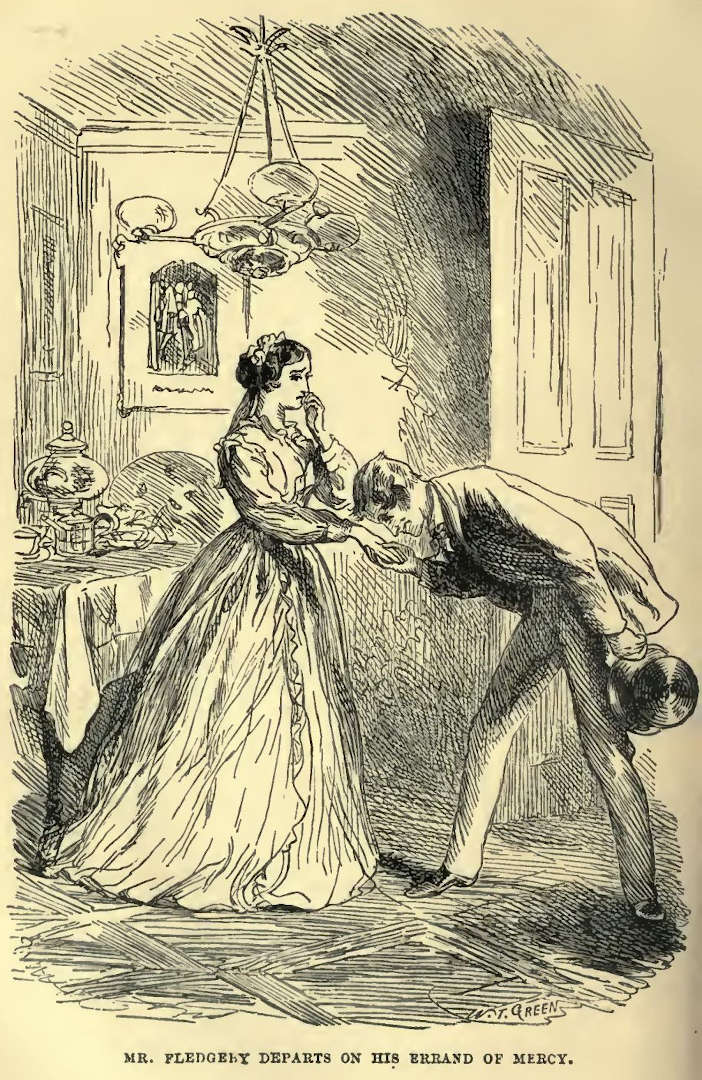
\includegraphics[scale=2.3]{03-12-01}

‘Noble action!’ said Mrs Lammle, extremely anxious to get rid of him.

‘It wasn’t what I was going to say,’ returned Fledgeby, who never would,
under any circumstances, accept a suggested expression, ‘but you’re very
complimentary. May I imprint a--a one--upon it? Good morning!’

‘I may depend upon your promptitude, dearest Mr Fledgeby?’

Said Fledgeby, looking back at the door and respectfully kissing his
hand, ‘You may depend upon it.’

In fact, Mr Fledgeby sped on his errand of mercy through the streets,
at so brisk a rate that his feet might have been winged by all the good
spirits that wait on Generosity. They might have taken up their station
in his breast, too, for he was blithe and merry. There was quite a fresh
trill in his voice, when, arriving at the counting-house in St Mary Axe,
and finding it for the moment empty, he trolled forth at the foot of the
staircase: ‘Now, Judah, what are you up to there?’

The old man appeared, with his accustomed deference.

‘Halloa!’ said Fledgeby, falling back, with a wink. ‘You mean mischief,
Jerusalem!’

The old man raised his eyes inquiringly.

‘Yes you do,’ said Fledgeby. ‘Oh, you sinner! Oh, you dodger! What!
You’re going to act upon that bill of sale at Lammle’s, are you? Nothing
will turn you, won’t it? You won’t be put off for another single minute,
won’t you?’

Ordered to immediate action by the master’s tone and look, the old man
took up his hat from the little counter where it lay.

‘You have been told that he might pull through it, if you didn’t go in
to win, Wide-Awake; have you?’ said Fledgeby. ‘And it’s not your game
that he should pull through it; ain’t it? You having got security, and
there being enough to pay you? Oh, you Jew!’

The old man stood irresolute and uncertain for a moment, as if there
might be further instructions for him in reserve.

‘Do I go, sir?’ he at length asked in a low voice.

‘Asks me if he is going!’ exclaimed Fledgeby. ‘Asks me, as if he didn’t
know his own purpose! Asks me, as if he hadn’t got his hat on ready!
Asks me, as if his sharp old eye--why, it cuts like a knife--wasn’t
looking at his walking-stick by the door!’

‘Do I go, sir?’

‘Do you go?’ sneered Fledgeby. ‘Yes, you do go. Toddle, Judah!’



